\documentclass[lecture,12pt,]{pcms-l}
\input preamble.tex

% For faster processing, load Matlab syntax for listings
\definecolor{MyDarkGreen}{rgb}{0.0,0.4,0.0}
\lstloadlanguages{Matlab}%
\lstset{language=Matlab,
        frame=single,
        basicstyle=\small\ttfamily,
        keywordstyle=[1]\color{Blue}\bf,
        keywordstyle=[2]\color{Purple},
        keywordstyle=[3]\color{Blue}\underbar,
        identifierstyle=,
        commentstyle=\usefont{T1}{pcr}{m}{sl}\color{MyDarkGreen}\small,
        stringstyle=\color{Purple},
        showstringspaces=false,
        tabsize=5,
        % Put standard MATLAB functions not included in the default
        % language here
        morekeywords={xlim,ylim,var,alpha,factorial,poissrnd,normpdf,normcdf},
        % Put MATLAB function parameters here
        morekeywords=[2]{on, off, interp},
        % Put user defined functions here
        morekeywords=[3]{FindESS},
        morecomment=[l][\color{Blue}]{...},
        numbers=left,
        firstnumber=1,
        numberstyle=\tiny\color{Blue},
        stepnumber=0
        }

% Only the next five fields need to be edited.
\newcommand{\lecAuth}{R.A. de Callafon}
\newcommand{\scribe}{Thomas Denewiler}
\newcommand{\authEmail}{callafon@ucsd.edu}
\newcommand{\scribeEmail}{tdenewiler@gmail.com}
\newcommand{\course}{MAE 283: Parameter Estimation}
\newcommand{\lectureNum}{5}

\address{Department of Mechanical and Aerospace Engineering, University of California, San Diego}

% Adds a hyperlink to an email address.
\newcommand{\mailto}[2]{\href{mailto:#1}{#2}}

% These commands set the document properties for the PDF output. Needs the hyperref package.
\hypersetup
{
    colorlinks,
    linkcolor={black},
    citecolor={black},
    filecolor={black},
    urlcolor={black},
    pdfauthor={\scribe <\mailto{\scribeEmail}{\scribeEmail}>},
    pdfsubject={\course},
    pdftitle={Lecture \lectureNum},
    pdfkeywords={UC San Diego, Parameter Estimation, System Identification},
    pdfstartpage={1},
}

% Includes a figure
% The first parameter is the label, which is also the name of the figure
%   with or without the extension (e.g., .eps, .fig, .png, .gif, etc.)
%   IF NO EXTENSION IS GIVEN, LaTeX will look for the most appropriate one.
%   This means that if a DVI (or PS) is being produced, it will look for
%   an eps. If a PDF is being produced, it will look for nearly anything
%   else (gif, jpg, png, et cetera). Because of this, when I generate figures
%   I typically generate an eps and a png to allow me the most flexibility
%   when rendering my document.
% The second parameter is the width of the figure normalized to column width
%   (e.g. 0.5 for half a column, 0.75 for 75% of the column)
% The third parameter is the caption.
\newcommand{\scalefig}[3]{
  \begin{figure}[ht!]
    % Requires \usepackage{graphicx}
    \centering
	\fbox{
	    \includegraphics[width=#2\columnwidth]{#1}
	}
    %%% I think \captionwidth (see above) can go away as long as
    %%% \centering is above
    %\captionwidth{#2\columnwidth}%
    \caption{#3}
    \label{#1}
  \end{figure}}

% Includes a MATLAB script.
% The first parameter is the label, which also is the name of the script
%   without the .m.
% The second parameter is the optional caption.
\newcommand{\matlabscript}[2]
  {\begin{itemize}\item[]\lstinputlisting[caption=#2,label=#1]{#1.m}\end{itemize}}

% Example environment.
\newtheoremstyle{example}{\topsep}{\topsep}	%
     {}%         Body font
     {}%         Indent amount (empty = no indent, \parindent = para indent)
     {\bfseries}% Thm head font
     {}%        Punctuation after thm head
     {\newline}%     Space after thm head (\newline = linebreak)
     {\thmname{#1}\thmnumber{ #2}\thmnote{ #3}}%         Thm head spec

   \theoremstyle{example}
   \newtheorem{example}{Example}[section]

% A command to show a vector norm that will have the pipe signs scale with the contents.
\newcommand{\vectornorm}[1]{\left|\left|#1\right|\right|}

% Commands for time and frequency integrals over infinty, cos and sin.
\newcommand{\tint}{\int_{t=-\infty}^\infty}
\newcommand{\fint}{\int_{\omega=-\infty}^\infty}
\newcommand{\tauint}{\int_{\tau=0}^\infty}
\newcommand{\w}{\omega}
\newcommand{\wo}{\omega_0}
\newcommand{\ejwt}{e^{j\omega t}}
\newcommand{\emjwt}{e^{-j\omega t}}
\newcommand{\dt}{\Delta T}
\newcommand{\tausum}{\sum_{\tau=-\infty}^\infty}
\newcommand{\ksum}{\sum_{k=-\infty}^\infty}
\newcommand{\ruhat}{\hat{R}_u^N(\tau)}
\newcommand{\ryuhat}{\hat{R}_{yu}^N(\tau)}
\newcommand{\phiuhat}{\hat{\phi}_u^N(\omega)}


%%%%%%%%%%%%%%%%%%%%%%%%%%%%%%%%%%%%%%%%%%%%%%%%%%%%%%%%%%%%%


\begin{document}
\mainmatter
\setcounter{page}{1}

\lectureseries[\course]{\course}

\auth[R.A. de Callafon]{Lecturer: \lecAuth\\ Scribe: \scribe}
\date{October 8, 2009}

\setaddress

% the following hack starts the lecture numbering at 5
\setcounter{lecture}{4}
\setcounter{chapter}{4}

\lecture{Estimating Covariance and Spectral Functions}

\section{Covariance and Spectral Functions}
The covariance and spectral density functions are defined as
\begin{definition}{Covariance and Spectral Density}

Auto-covariance function
\begin{align}
\label{eq:autocov}
R_u(\tau) = \bar{E}\{u(t)u(t-\tau)\}
\end{align}
Cross-covariance function
\begin{align}
\label{eq:xcov}
R_{yu}(\tau) = \bar{E}\{y(t)u(t-\tau)\}
\end{align}
Auto-spectral density function
\begin{align}
\label{eq:autospec}
\phi_u(\w) = \tausum R_u(\tau)e^{-j\w\tau} = \mathcal{F}\{R_u(\tau)\}
\end{align}
Cross-spectral density function
\begin{align}
\label{eq:xspec}
\phi_{yu}(\w) = \mathcal{F}\{R_{yu}(\tau)\}
\end{align}
\end{definition}

\subsection{Applications}
Suppose a system is given by $y(t) = G_0(q)u(t)+w(t)$ and assume that $u\perp v$. Then
$$R_{yu}(\tau) = g_0(k)$$
if the sequence of inputs $\{u(t)\}$ is white noise and says that we can get the impulse response, or Markov, parameters from the cross-covariance of the input and output. We can also find the other values in (\ref{eq:autocov} - \ref{eq:xspec}) as
\begin{align*}
R_{yu}(\tau) &= G_0(q)R_u(\tau) \\
\phi_{yu}(\w) &= G_0(e^{j\w})\phi_u(\w) \\
\phi_y(\w) &= |G_0(e^{j\w})|^2\phi_u(\w) + \phi_v(\w)
\end{align*}

\subsection{Properties}
Notice that $R_u(\tau)=R_u(-\tau)$. The product $u(t)u(t-\tau)$ remains the same and implies that the auto-covariance function is symmetric about $\tau=0$.

The auto-spectral density function is real-valued, $\phi_u(\w) = \mathcal{F}\{R_u(\tau)\}\in\mathbb{R}$. Any Fourier transform is real when the signal is symmetric.

The cross-covariance function is \textit{not} symmetric, $R_{yu}(\tau)\neq R_{yu}(-\tau)$.

The cross-spectral density function is complex-valued in general,
$$\phi_{yu}(\w) = \mathcal{F}\{R_{yu}(\tau)\}\in\mathbb{C} \rightarrow \phi_{yu}(\w)\in\mathbb{C} = G_0(e^{j\w})\in\mathbb{C} \cdot \phi_u(\w)\in\mathbb{R}$$

Let $y(t) = G_0(q)u(t)+v(t)$, with $\{u(t)\}=\text{ white noise}$ and $u\perp v$. This defines a causal system. In a causal system $R_{yu}(-\tau)=0$. This means that the system output is not reacting to an input \textit{before} the input is applied. Recall that $R_{yu}(-\tau)=g_0(k)$ because the input is white noise. The $g_0(k)$ values represent the impulse response and they \textit{must} be zero for input that has not occurred, as represented by $t=-\tau$.

\section{Finite-time Estimates}
In the textbook, Ljung calls this non-parametric identification. The goal is to find estimates of (\ref{eq:autocov} - \ref{eq:xspec}). We have to find estimates for these values because they are defined assuming that there are an infite number of samples and we will only have a finite number of samples.

\subsection{Correlation analysis}
\begin{align*}
R_{yu}(\tau) &= G_0(q)R_u(\tau) \Rightarrow R_u(\tau) = \begin{cases} \lambda, & \tau=0 \\ 0, & |\tau|\neq 0 \end{cases} \\
&= \lambda g_00(\tau) \Rightarrow g_0(\tau) = \frac{R_{yu}(\tau)}{\lambda}
\end{align*}
Therefore, we need to find estimates for $R_{yu}(\tau)$ and $R_u(\tau)$ to find the impulse response coefficients.

\subsection{Estimation of Covariance Functions}
From (\ref{eq:autocov}) we have
$$R_u(\tau) = \bar{E}\{u(t)u(t-\tau)\} = \lim_{N\to\infty}\frac{1}{N}\sum_{t=1}^N E\{u(t)u(t-\tau)\}$$
A proposed form of the estimate is
$$\hat{R}_u^N(\tau) = \frac{1}{N}\sum_{t=1}^u(t)u(t-\tau)$$
The idea is that we will leave out the estimator operation because we do not know what it is. We hope that taking enough samples and averaging them will lead to a good estimate of the true covariance.

Looking at the expected value of this proposed covariance estimate, we would like it to have the property
$$\lim_{N\to\infty} E\{\ruhat\} = R_u(\tau) \text{ w.p. } 1$$
If that is the case then it is called a ``consistent'' estimate. The result is actually
\begin{align}
\label{eq:autocovest}
E\{\ruhat\} = \frac{N-|\tau|}{N}R_u(\tau)
\end{align}
where $\frac{N-|\tau|}{N}$ is a weighting factor with the property that $\lim_{N\to\infty}E\{\ruhat\}=R_u(\tau)$. Notice that the proposed estimate is biased by the weighting term, but it is asymptotically stable. Also, the estimate gets better as more data is sampled.

\subsection{Unbiased Estimate of $R_u(\tau)$}
To get an unbiased estimate of $R_u(\tau)$ we use
$$\hat{\hat{R}}_u^N(\tau) = \frac{1}{N-|\tau|}\sum_{t=1}^Nu(t)u(t-\tau)$$
We can only sum samples over $N-|\tau|$. In the end, we will use the biased estimate anyway! Later we will look at the math to show why. It is mostly because over a smaller number of samples we do not trust the estimate that much and we want to capture that information. As the time-shift $\tau$ gets larger Figure \ref{fig:05timeShift} shows that we have fewer samples to use when calculating the covariance. Figure \ref{fig:05triWindow} shows the triangular window that represents the weighting factor and shows how the weighting factor forces the estimate to zero for large values of $\tau$. In \textsc{Matlab} the function \texttt{xcorr} can be used to find the covariance estimate by using \texttt{xcorr(u,u,'biased')}.
\begin{figure}[ht!]
	\centering
	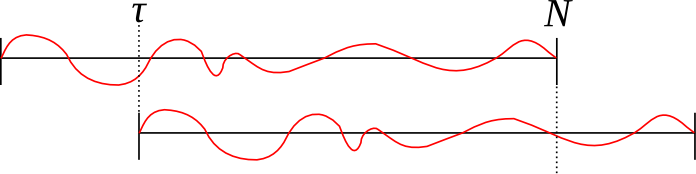
\includegraphics[width=.6\textwidth]{images/05timeShift}
	\caption{Effect of time-shifting a signal.}
	\label{fig:05timeShift}
\end{figure}

\begin{figure}[ht!]
	\centering
	\includegraphics[width=.3\textwidth]{images/05triWindow}
	\caption{Triangular window from weighting factor.}
	\label{fig:05triWindow}
\end{figure}

\subsection{Covariance of Estimator}
\begin{align*}
E\{u(t)u(t-\tau)\} &= \begin{cases} \lambda, & \tau=0 \\ R_u(\tau), & |\tau|\neq 0 \end{cases} \\
\text{cov}\{\ruhat,\hat{R}_u^N(\tau+k)\} &\sim \frac{1}{N}\sum_{m=-\infty}^\infty R_u(m)R_u(m+k) + R_u(m+\tau+k)R_u(m-\tau)
\end{align*}
Let $m=k$, then
\begin{align*}
\text{cov}\{\ruhat,\hat{R}_u^N(\tau+k)\} &\sim \frac{1}{N}\underbrace{\sum_{m=-\infty}^\infty R_u^2(m) + R_u(m+\tau)R_u(m-\tau)}_C
\end{align*}
Note that since $\{u(t)\}$ is quasi-stationary $R_u(\tau)\to0$ eventually. This leads to
\begin{align*}
\text{cov}\{\ruhat\ruhat\} &\sim \mathcal{O}(\frac{1}{N}) < \frac{C}{N} \\
\lim_{N\to\infty}\text{cov}\{\ruhat\ruhat\} &= 0
\end{align*}
This means that the variance goes to zero with probability $1$. See Figure \ref{fig:05estDist}.
\begin{figure}[ht!]
	\centering
	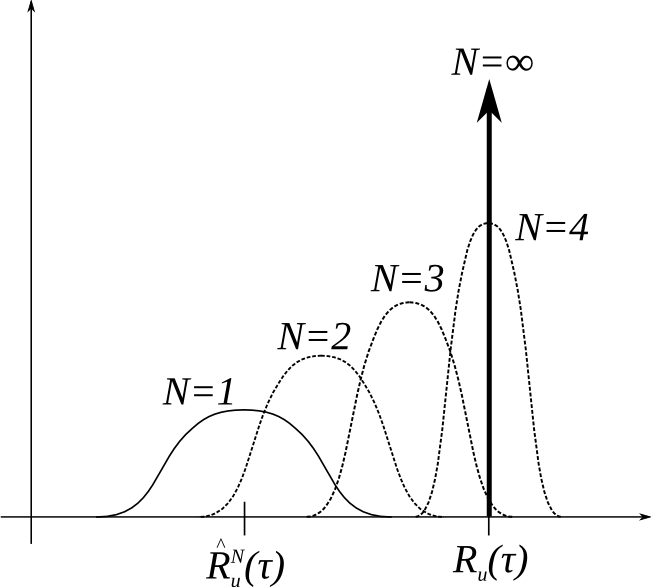
\includegraphics[width=.4\textwidth]{images/05estDist}
	\caption{Distributions of estimators as $N\to\infty$.}
	\label{fig:05estDist}
\end{figure}

\begin{example}
\begin{align*}
\ruhat &= \begin{cases} \frac{1}{N}\sum_{t=1}^Nu(t)u(t-\tau), & |\tau|\leq N-1 \\ 0, & |\tau|\geq N \end{cases} \\
&\text{use DTFT} \\
\sum_{\tau=-\infty}^\infty\ruhat e^{-j\w\tau} &= \phiuhat = \frac{1}{N}\left|U_N(\w)\right|^2 \triangleq \text{ periodogram} \\
&\text{use DTFT} \\
U_N(\w) &= \sum_{t=0}^{N-1}u(t)e^{-j\w t}
\end{align*}
Later it will be shown why $\phiuhat$ is \textit{not} a good estimate. Now we can compute $\ruhat$ using (\ref{eq:autocovest}) or
\begin{align*}
\mathcal{F}\{u(t)\} &= U_N(\w) \\
\mathcal{F}^{-1}\{U_N(\w)\overline{U_N(\w)}\} &= \ruhat
\end{align*}
The benefit of this last representation is that Fourier transforms can be \textit{very} fast to compute using digital systems and this is important when there are a large number of estimates to find.
\end{example}
$\lozenge$

\subsection{Cross-covariance Functions}
This analysis is very similar to that for the auto-covariance functions. From (\ref{eq:xcov}) we have
\begin{align*}
R_{yu}(\tau) = \bar{E}\{y(t)u(t-\tau)\} &= \lim_{N\to\infty}\frac{1}{N}\sum{t=1}^N E\{y(t)u(t-\tau)\} \\
\ryuhat &= \frac{1}{N}\sum_{t=1}^Ny(t)u(t-\tau) \\
E\{R_{yu}(\tau)\} &= \frac{N-|\tau|}{N}R_{yu}(\tau) \sim \mathcal{O}(\frac{1}{N}) \\
\lim_{N\to\infty}\ryuhat &= R_{yu}(\tau) \text{ w.p. } 1
\end{align*}
The last equality implies that there is no variance in the estimate when an infinite number of samples are available. It is a stronger statement than
$$\lim_{N\to\infty}E\{\ryuhat\} = R_{yu}(\tau)$$
which has a variance that could be large. In \textsc{Matlab} the cross-covariance between two signals can be found using \texttt{xcorr(u,y,'unbiased')}, where the order is input then output. We can also find the cross-covariance using fast Fourier transforms by using
\begin{align*}
\mathcal{F}\{u(t)\} &= U_N(\w) \\
\mathcal{F}\{y(t)\} &= Y_N(\w) \\
\mathcal{F}^{-1}\{Y_N(\w)\overline{U_N(\w)}\} &= R_{yu}(\tau)
\end{align*}

\subsection{Applications}
Using the system $y(t) = G_0(q)u(t)+v(t)$ we have
\begin{align*}
\sum_{t=1}^Ny(t)u(t-\tau) &= G_0(q)\frac{1}{N}\sum_{t=1}^Nu(t)u(t-\tau) + \frac{1}{N}\sum_{t=1}^Nv(t)u(t-\tau) \\
\ryuhat &= G_0(q)\ruhat + \hat{R}_{vu}^N(\tau)
\end{align*}
If $u\perp v$ then $R_{vu}(\tau)=0$, but $\hat{R}_{vu}^N(\tau)\neq 0$ because there is some bias that we will call $v(t)$. Also, if $\{u(t)\}$ is white noise then $R_u(\tau)$ will be a $\delta$-function, but $\ruhat$ will not be a perfect $\delta$-function. See Figure \ref{fig:05xcov}. This leads to
\begin{align*}
\ryuhat &= \hat{g}_0(\tau) \\
\lim_{N\to\infty}E\{\ryuhat\} &= g_0(\tau)
\end{align*}
If $v(t)=0$ then $\ryuhat=\hat{g}_0(\tau)$ is \textit{still} an estimate because we do not have a perfect $\delta$-function so we do not get a perfect impulse response, but it typically gives a pretty close estimate of the parameters $g_0(\tau)$.
\begin{figure}[ht!]
	\centering
	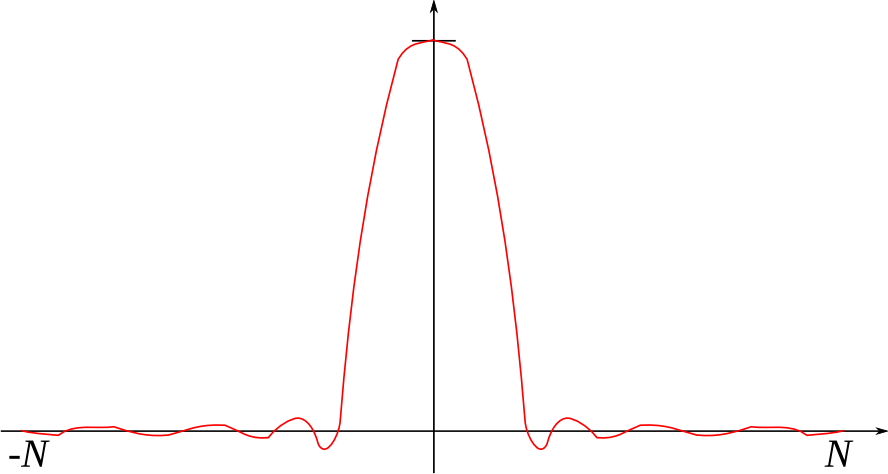
\includegraphics[width=.5\textwidth]{images/05xcov}
	\caption{Estimated covariance when the input is not a perfect $\delta$-function.}
	\label{fig:05xcov}
\end{figure}

\section{Finite Impulse Response}
Assume $G_0(q) = \sum_{k=0}^ng_0(k)q^{-k}$. This means that $G_0(q)$ is the finite impulse response (FIR) because we are only looking at $n$ samples, not an infinte amount of samples.

When $\{u(t)\}$ is white noise how do we estimate the parameters $g_0(k)$? We cannot use $\hat{g}_0(k) = \hat{R}_{yu}^N(k)$ because $R_u(\tau)\neq \delta_d(\tau)$, where $\delta_d(\tau)$ is a $\delta$-function. However, we can use
$$R_{yu}(\tau) = G_0(q)R_u(\tau) = \sum_{k=0}^ng_0(k)R_u(\tau-k)$$
Solving for the first few values of $k$ gives
\begin{align*}
R_{yu}(0) &= g_0(0)R_u(0) + g_0(1)R_u(-1) + g_0(2)R_u(-2) + \cdots + g_0(n)R_u(-n) \\
&= g_0(0)R_u(0) + g_0(1)R_u(1) + g_0(2)R_u(2) + \cdots + g_0(n)R_u(n) \\
R_{yu}(1) &= g_0(0)R_u(1) + g_0(1)R_u(0) + g_0(2)R_u(-1) + \cdots + g_0(n)R_u(-n) \\
&= g_0(0)R_u(1) + g_0(1)R_u(0) + g_0(2)R_u(1) + \cdots + g_0(n)R_u(n)
\end{align*}
where we use the symmetry property of $R_u(k)$. Writing this in matrix form gives
\begin{align*}
\left[\begin{array}{c}
R_{yu}(0) \\ R_{yu}(1) \\ \vdots \\ R_{yu}(n)
\end{array}\right] =
\left[\begin{array}{c c c c c}
R_u(0) & R_u(1) & R_u(2) & \cdots & R_u(n) \\
R_u(1) & R_u(0) & R_u(1) & \cdots & R_u(n-1) \\
R_u(2) & R_u(1) & R_u(0) & \cdots & R_u(n-2) \\
\vdots & \vdots & \vdots & \ddots & \vdots \\
R_u(n) & R_u(n-1) & R_u(n-2) & \cdots & R_u(0)
\end{array}\right]
\left[\begin{array}{c}
g_0(0) \\ g_0(1) \\ \vdots \\ g_0(n)
\end{array}\right]
\end{align*}
This can be rewritten as
$$\mathbf{R}_{yu} = \mathbf{R}_u\mathbf{\theta}$$
The matrix $\mathbf{R}_u$ is a symmetric Toeplitz matrix. When working with a finite number of samples we replace all of the values in the vectors and matrix with their estimated values and rearrange to get
\begin{align*}
\hat{\mathbf{R}}_{yu} = \hat{\mathbf{R}}_u\mathbf{\theta} \\
\mathbf{\theta} = \hat{\mathbf{R}}_u^{-1}\hat{\mathbf{R}}_{yu}
\end{align*}
This works even when the noise is not white. However, if the noise is white then $\hat{\mathbf{R}}_u$ is a diagonal matrix. Furthermore, if the noise has a variance $\sigma=1$ then $\hat{\mathbf{R}}_u=I$.

Notice that $\hat{\mathbf{R}}_u$ only depends on the input sequence $\{u(t)\}$. The invertibility of $\hat{\mathbf{R}}_u$ is a property of $\{u(t)\}$ and when it is possible is referred to as the ``persistence of excitation''. It is the responsibility of the engineer to create the input signal $\{u(t)\}$ such that $\hat{\mathbf{R}}_u$ is invertible.

\begin{example}
Suppose that the input signal is $u(t)=sin\w t$. Then we will only have $\text{rank}\{\hat{\mathbf{R}}_u\}=2$. We would only be able to estimate the first two parameters, $g_0(0)$ and $g_0(1)$. This is because a sinusoid only has two parameters, the frequency and amplitude or the frequency and phase shift. If two sinusoids are used as input then we could estimate four parameters.

Note that as $N\to\infty$ the parameters $g_0(k)$ go to the real values and are not estimated values.
\end{example}
$\lozenge$


\end{document}

%%%%%%%%%%%%%%%%%%%%%%%%%%%%%%%%%%%%%%%%%%%%%%%%%%%%%%%%%%%%%